\chapter[Aplicações à conservação]{Aplicações de SDM à Conservação}

\begin{objetivos}
	Ao final desta unidade, o estudante deverá compreender como modelos de distribuição de espécies podem apoiar decisões de conservação; integrar adequabilidade atual, estabilidade futura, incerteza e áreas protegidas; identificar áreas prioritárias para \textit{Dinizia excelsa}; avaliar lacunas de proteção; produzir mapas de prioridade espacial; e discutir aplicações em espécies ameaçadas, árvores gigantes, restauração ecológica e planejamento sistemático da conservação.
\end{objetivos}

\section{Introdução}

Modelos de Distribuição de Espécies são amplamente utilizados para apoiar estratégias de conservação, especialmente em cenários de mudanças climáticas, perda de habitat, fragmentação florestal e expansão de pressões antrópicas. Em aplicações conservacionistas, o objetivo não é apenas mapear onde uma espécie pode ocorrer, mas identificar regiões onde a adequabilidade ambiental, a estabilidade climática, a baixa incerteza e a proteção territorial convergem \parencite{margules2000systematic,moilanen2009spatial,franklin2023,guisan2017habitat,zurell2020benchmarking}.

Nesta unidade, integramos os produtos construídos nas unidades anteriores para desenvolver uma análise aplicada à conservação de \textit{Dinizia excelsa}. O foco está na construção de mapas de prioridade espacial baseados em evidências ecológicas, climáticas e modelagem preditiva.

\begin{conceito}[title={\faBook\quad SDM aplicado à conservação}]
	Em conservação, SDM deve ser interpretado como uma camada de evidência espacial. Ele deve ser combinado com informações sobre proteção territorial, conectividade, ameaça, incerteza e viabilidade ecológica.
\end{conceito}

\section{Critérios de priorização}

Nesta unidade, usamos cinco critérios principais:

\begin{itemize}
	\item alta adequabilidade atual;
	\item estabilidade futura;
	\item estabilidade paleoclimática;
	\item baixa incerteza integrada;
	\item presença ou ausência em áreas protegidas.
\end{itemize}

\begin{atencao}[title={\faExclamationTriangle\quad Prioridade não é apenas adequabilidade}]
	Uma área altamente adequada pode não ser prioritária se apresentar alta incerteza, forte extrapolação climática ou ausência de viabilidade de conservação. A priorização deve integrar múltiplas dimensões.
\end{atencao}

\section{Preparação dos dados espaciais}

\rscriptfile{scripts/unidade17/01_estrutura_pastas.R}

\rscriptfile{scripts/unidade17/02_preparar_camadas_conservacao.R}

\section{Prioridade climática atual}

\rscriptfile{scripts/unidade17/03_prioridade_climatica_atual.R}

\begin{figure}[H]
	\centering
	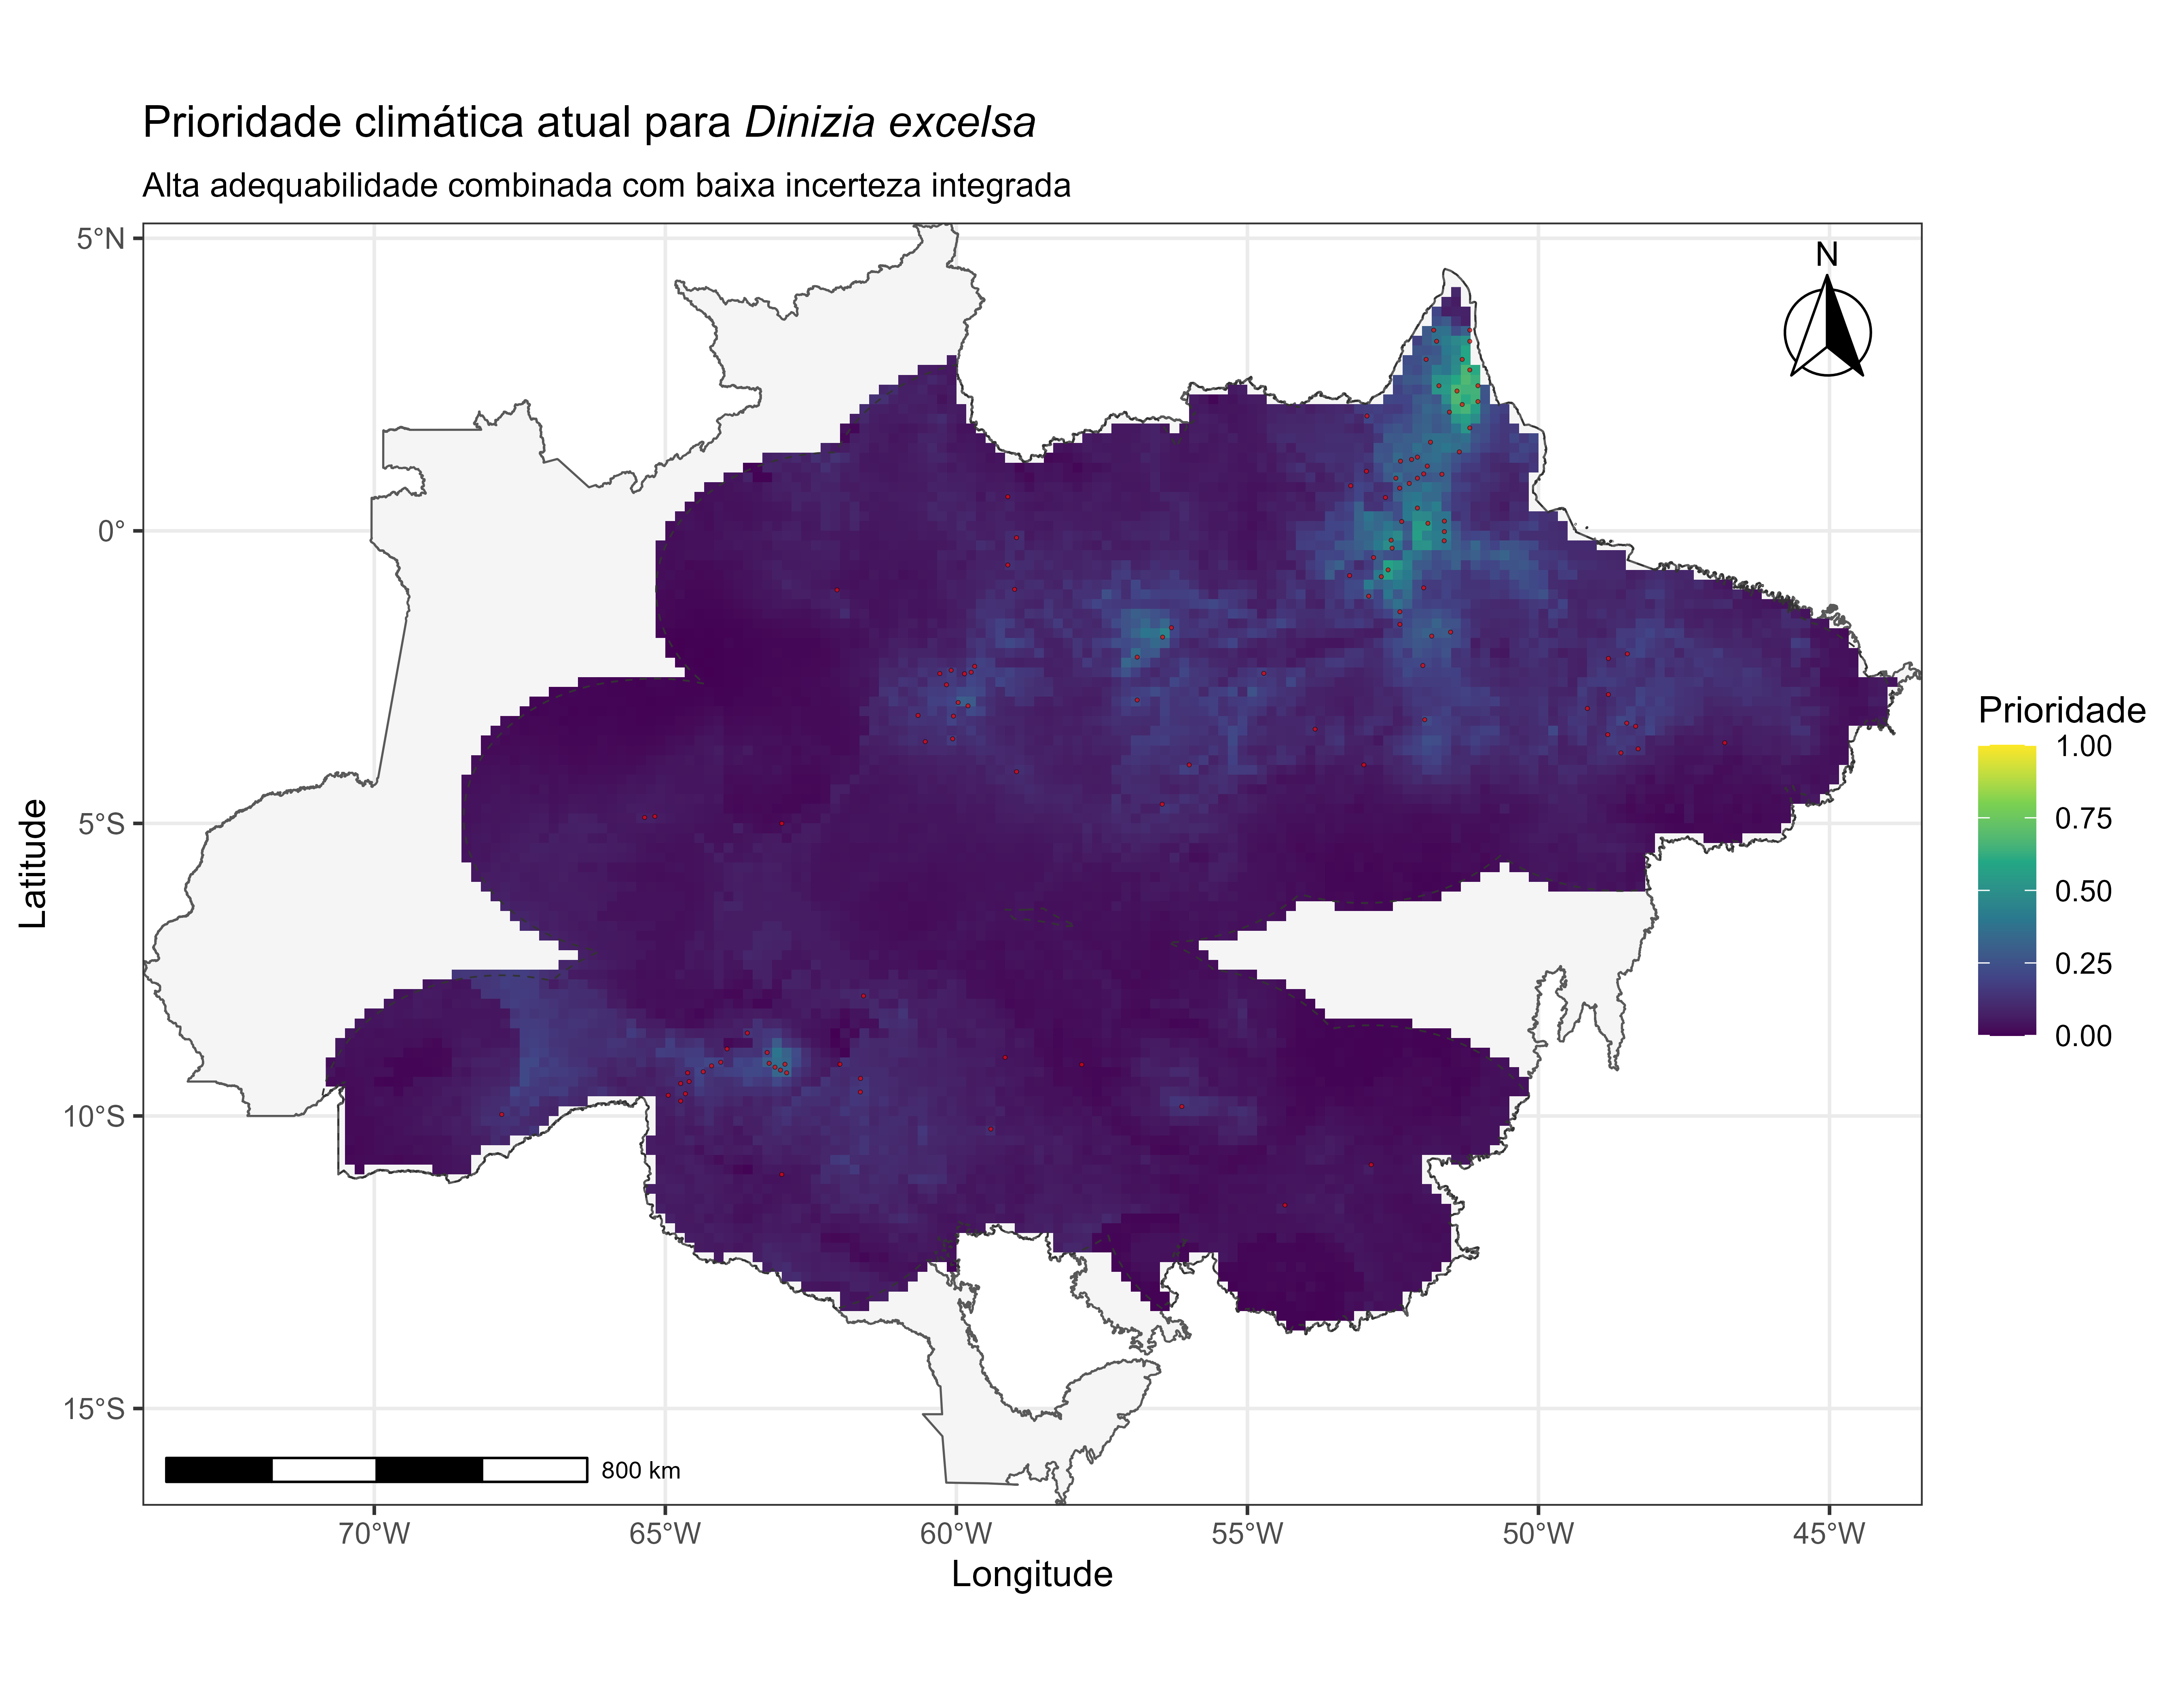
\includegraphics[width=0.88\textwidth]{figuras/unidade17/unidade17_prioridade_climatica_atual.png}
	\caption{Prioridade climática atual para \textit{Dinizia excelsa}, baseada em adequabilidade atual e incerteza integrada.}
	\label{fig:unidade17_prioridade_atual}
\end{figure}

\section{Estabilidade futura e conservação}

\rscriptfile{scripts/unidade17/04_estabilidade_futura_conservacao.R}

\begin{figure}[H]
	\centering
	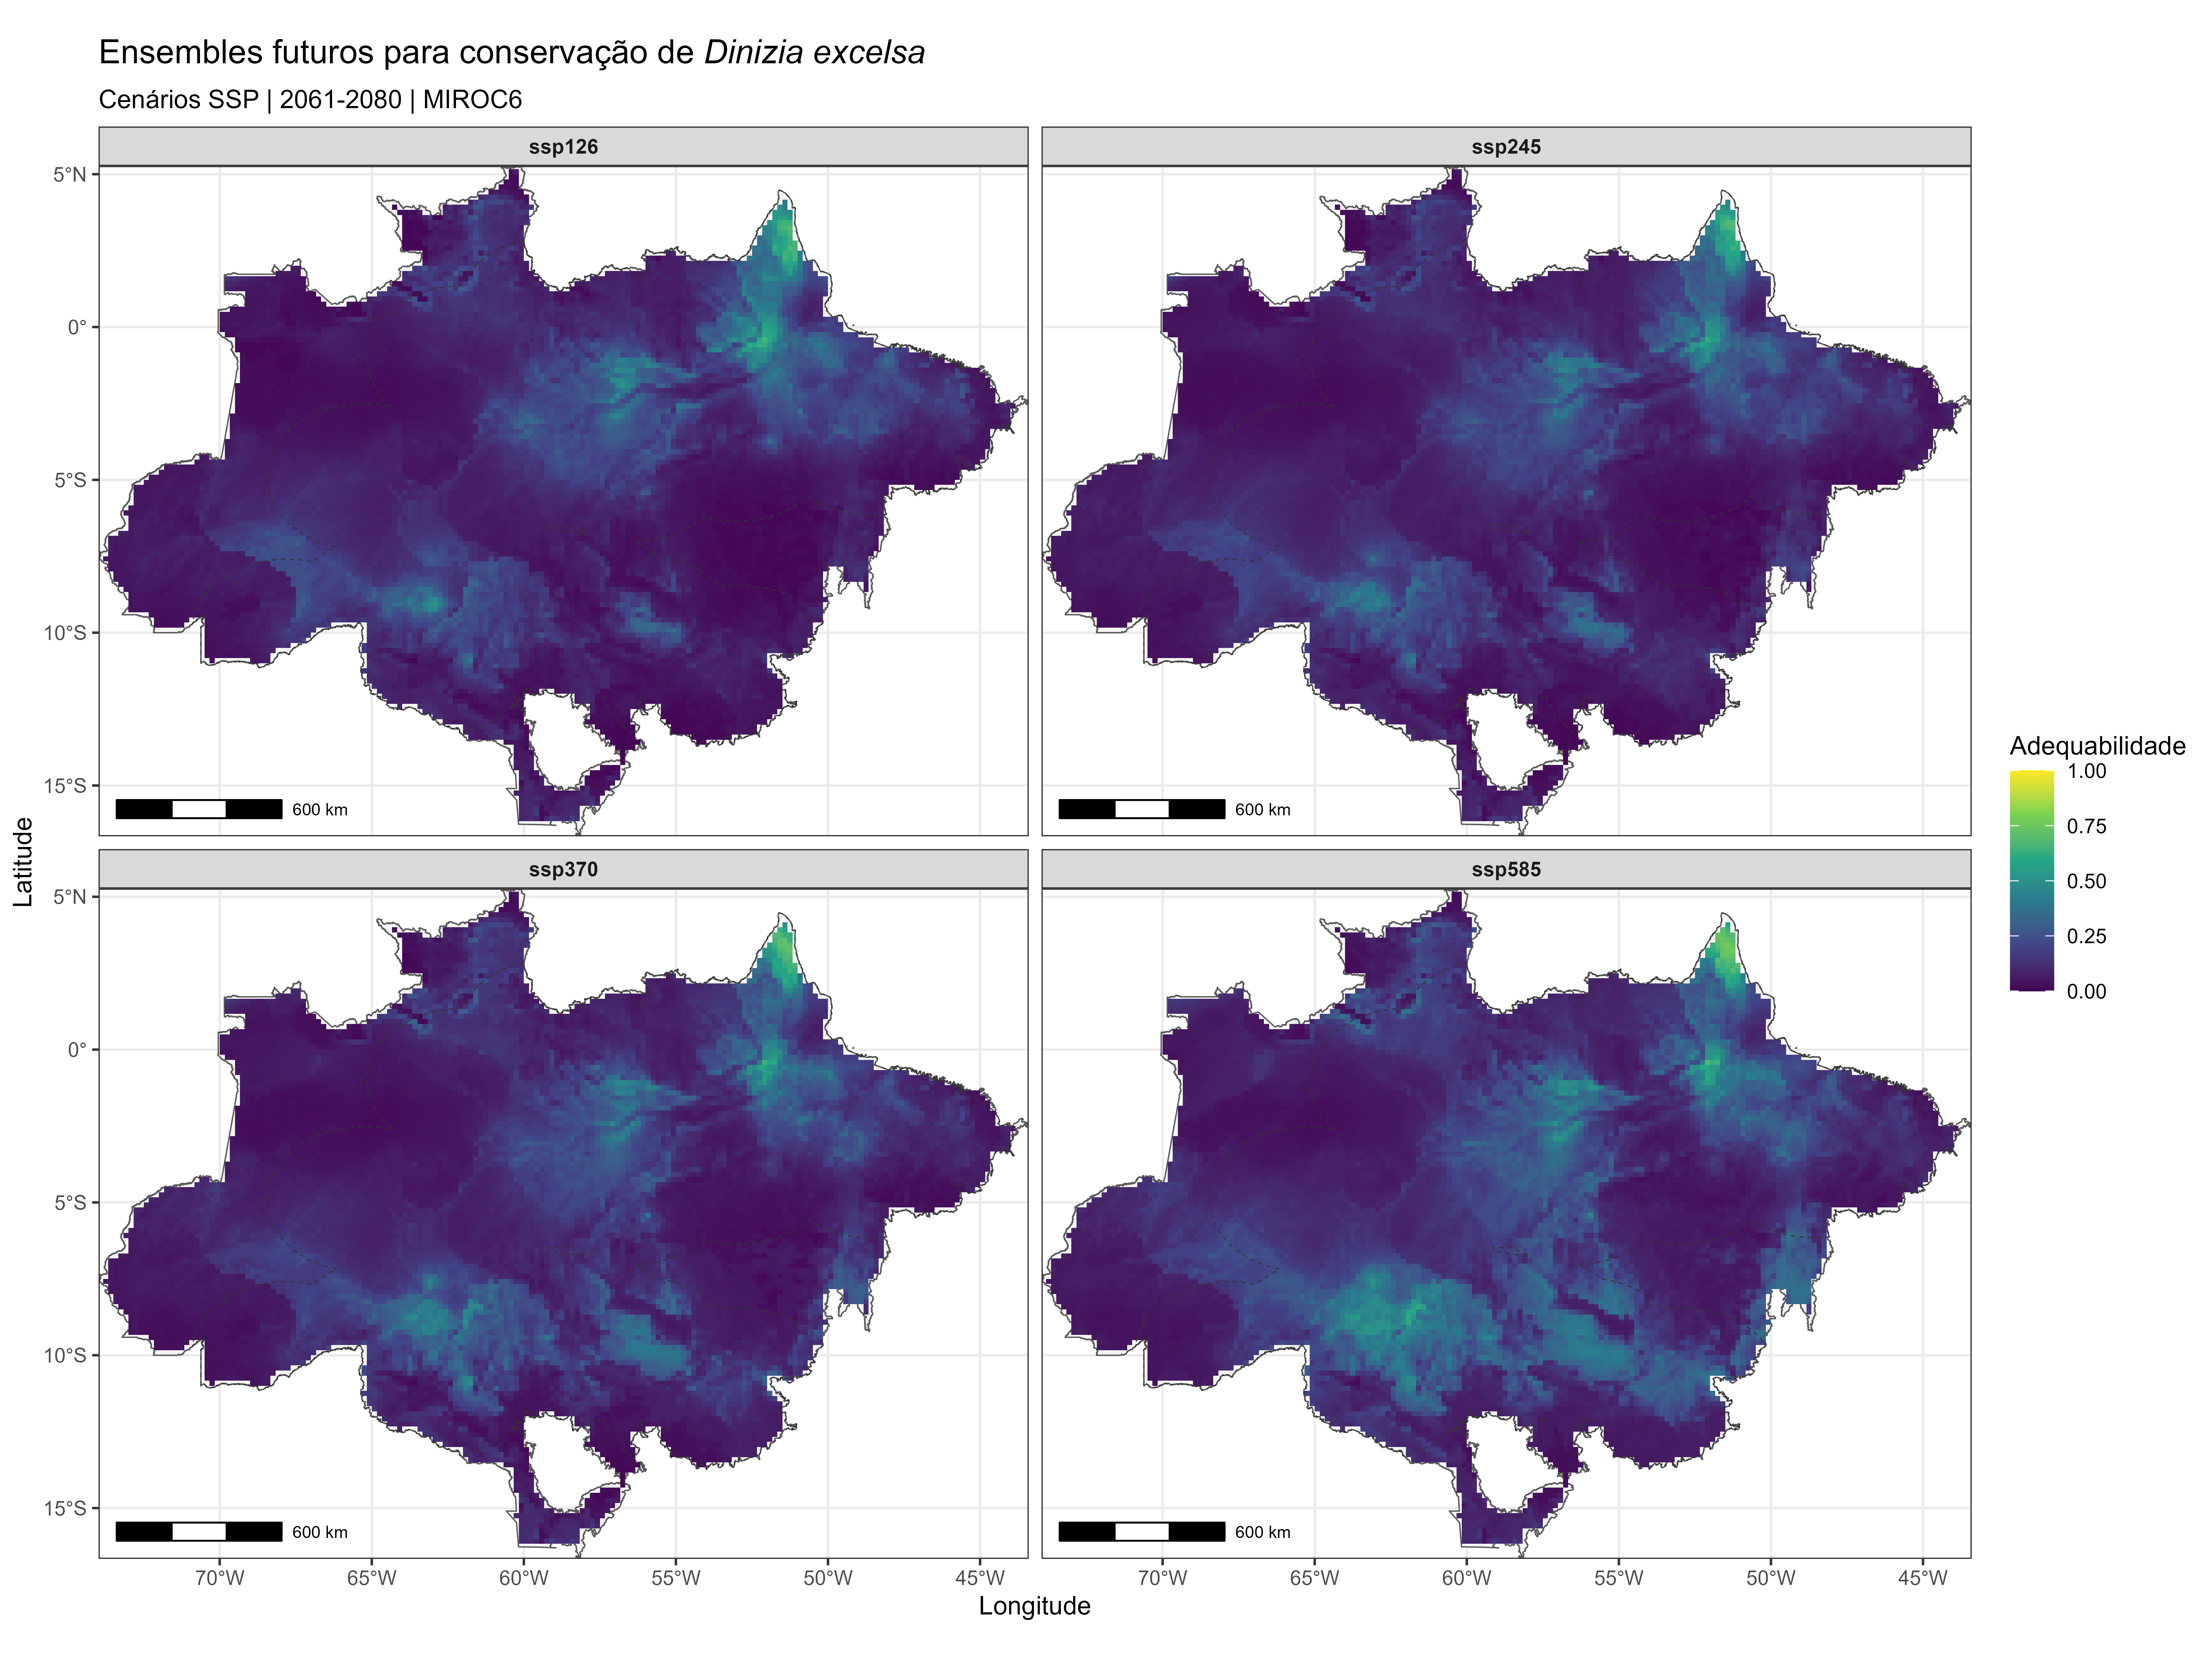
\includegraphics[width=0.96\textwidth]{figuras/unidade17/unidade17_estabilidade_futura_conservacao.png}
	\caption{Estabilidade futura de adequabilidade para \textit{Dinizia excelsa} sob cenários climáticos.}
	\label{fig:unidade17_estabilidade_futura}
\end{figure}

\section{Refúgios climáticos e estabilidade histórica}

\rscriptfile{scripts/unidade17/05_refugios_climaticos_conservacao.R}

\begin{figure}[H]
	\centering
	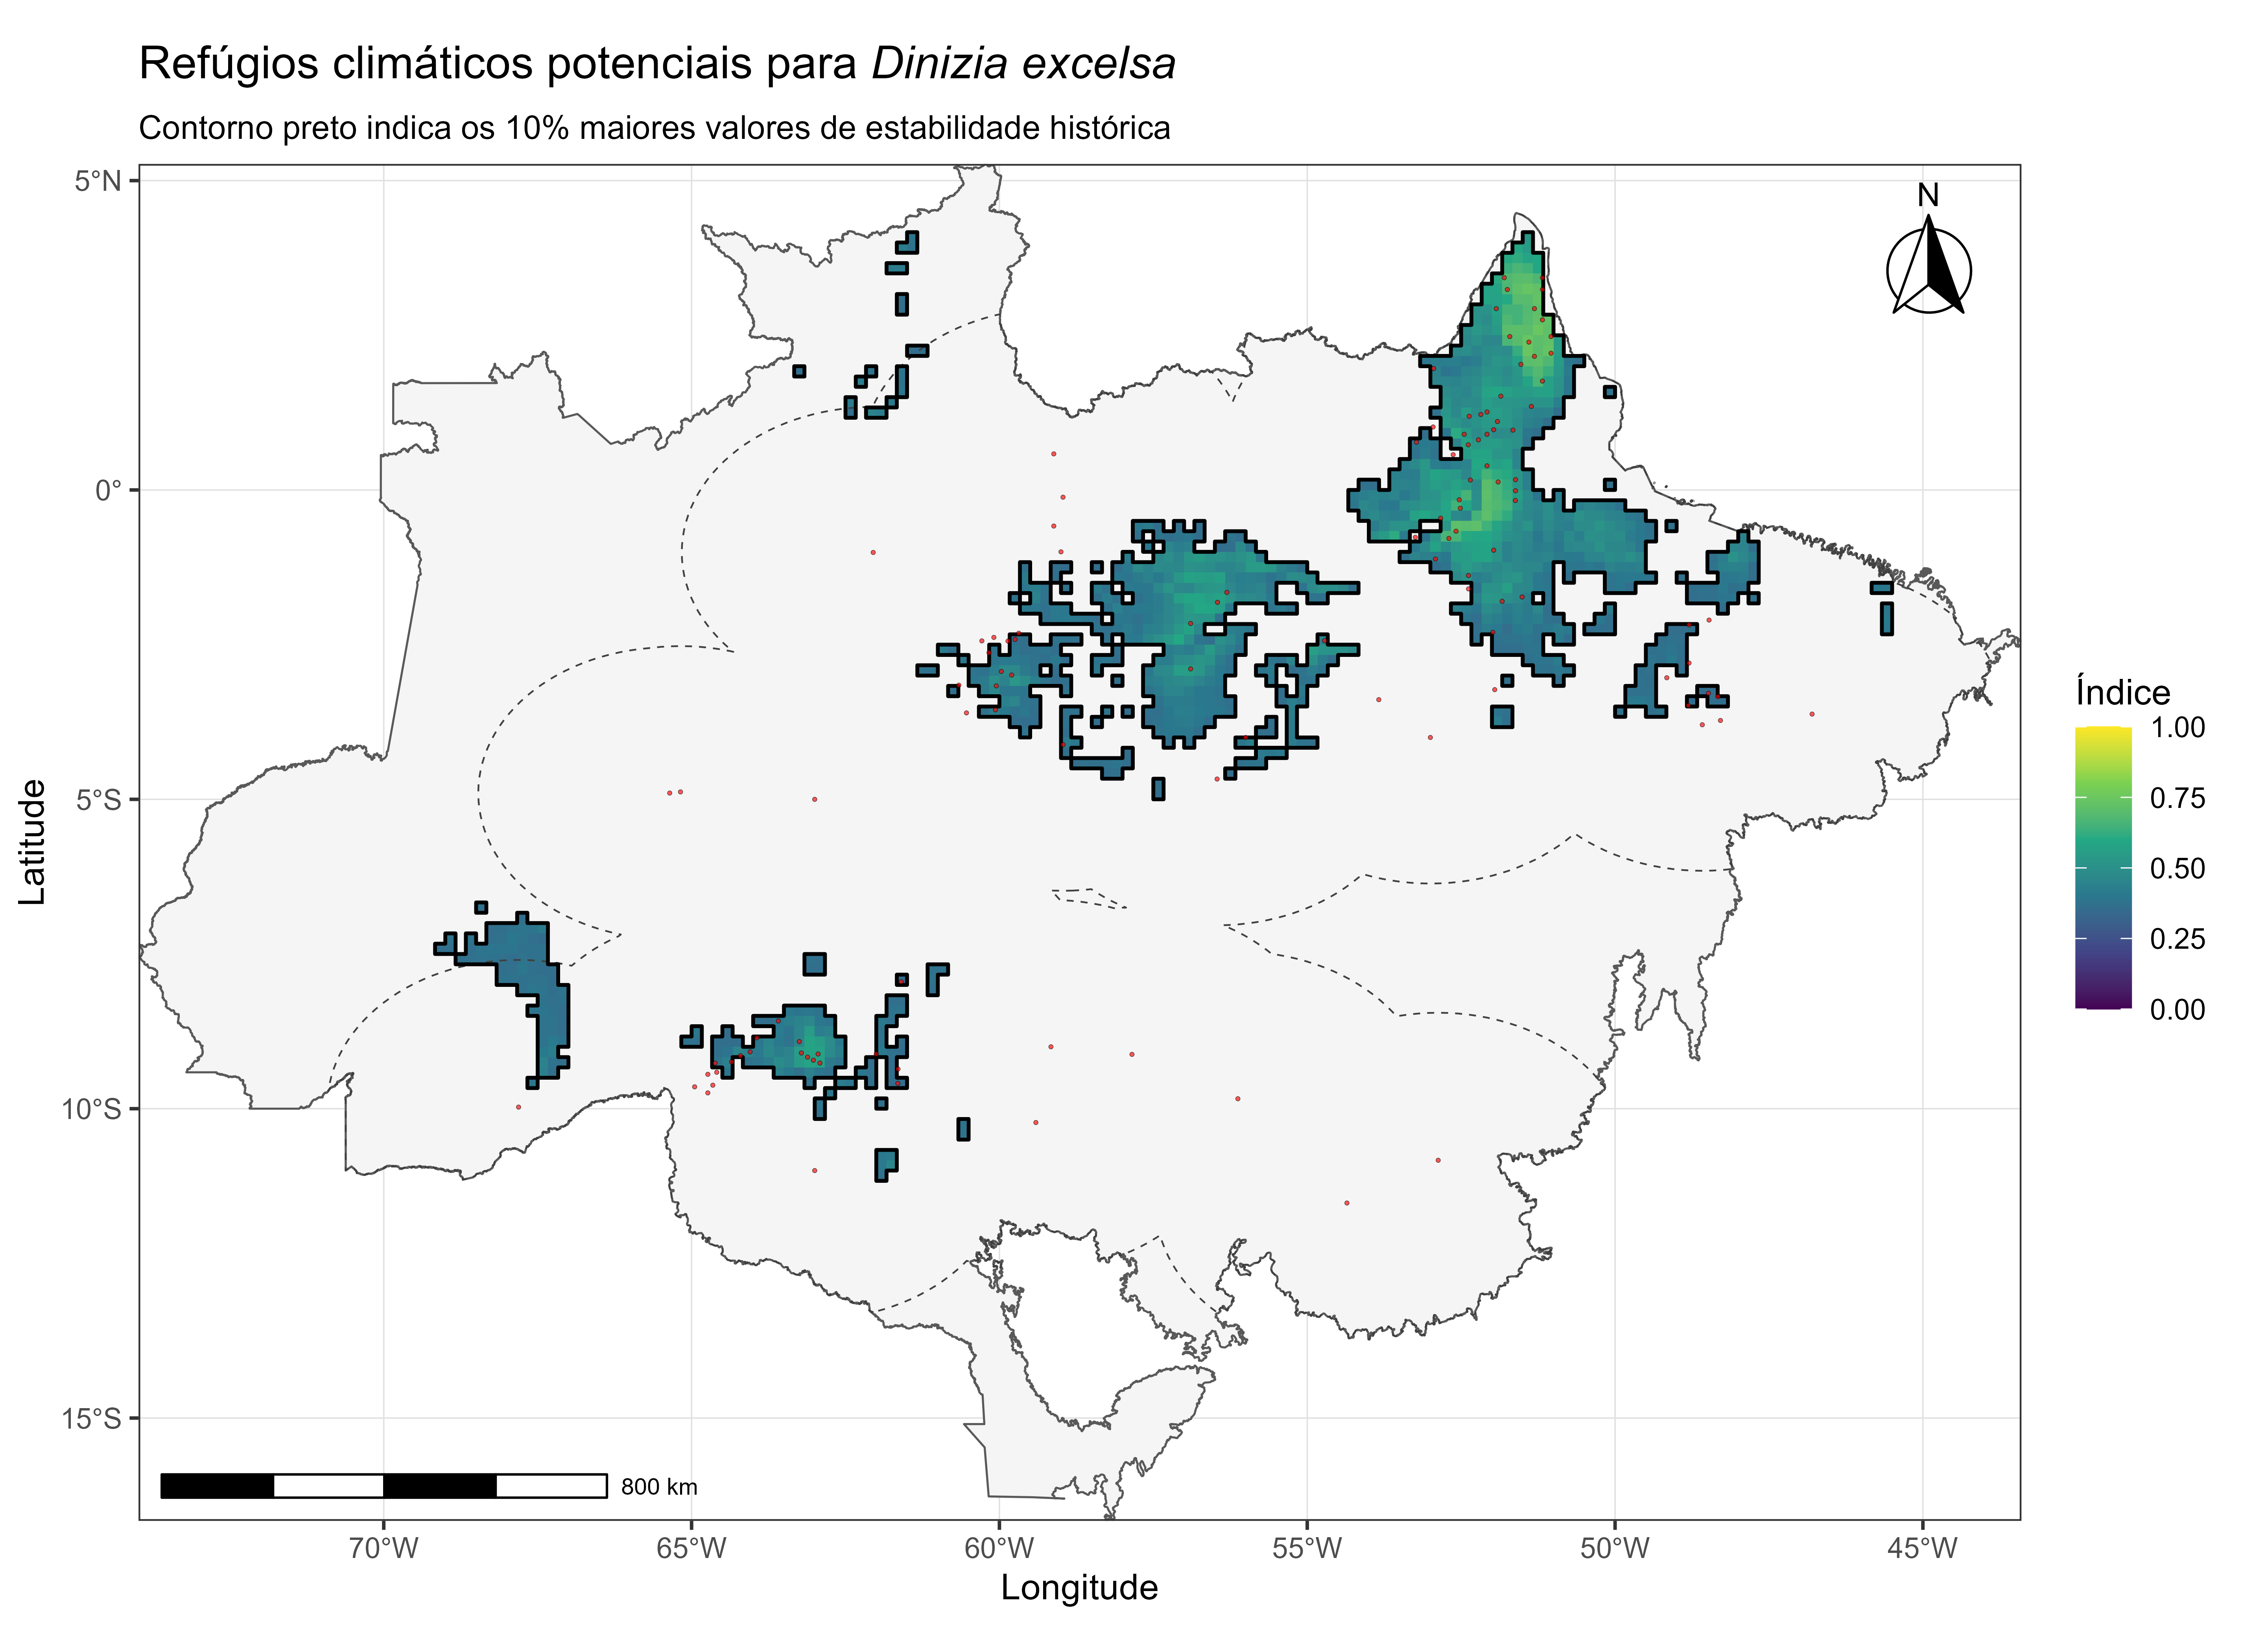
\includegraphics[width=0.96\textwidth]{figuras/unidade17/unidade17_refugios_climaticos.png}
	\caption{Áreas candidatas a refúgios climáticos para \textit{Dinizia excelsa}, integrando estabilidade atual e paleoclimática.}
	\label{fig:unidade17_refugios}
\end{figure}

\section{Lacunas de proteção}

\rscriptfile{scripts/unidade17/06_lacunas_protecao.R}

\begin{figure}[H]
	\centering
	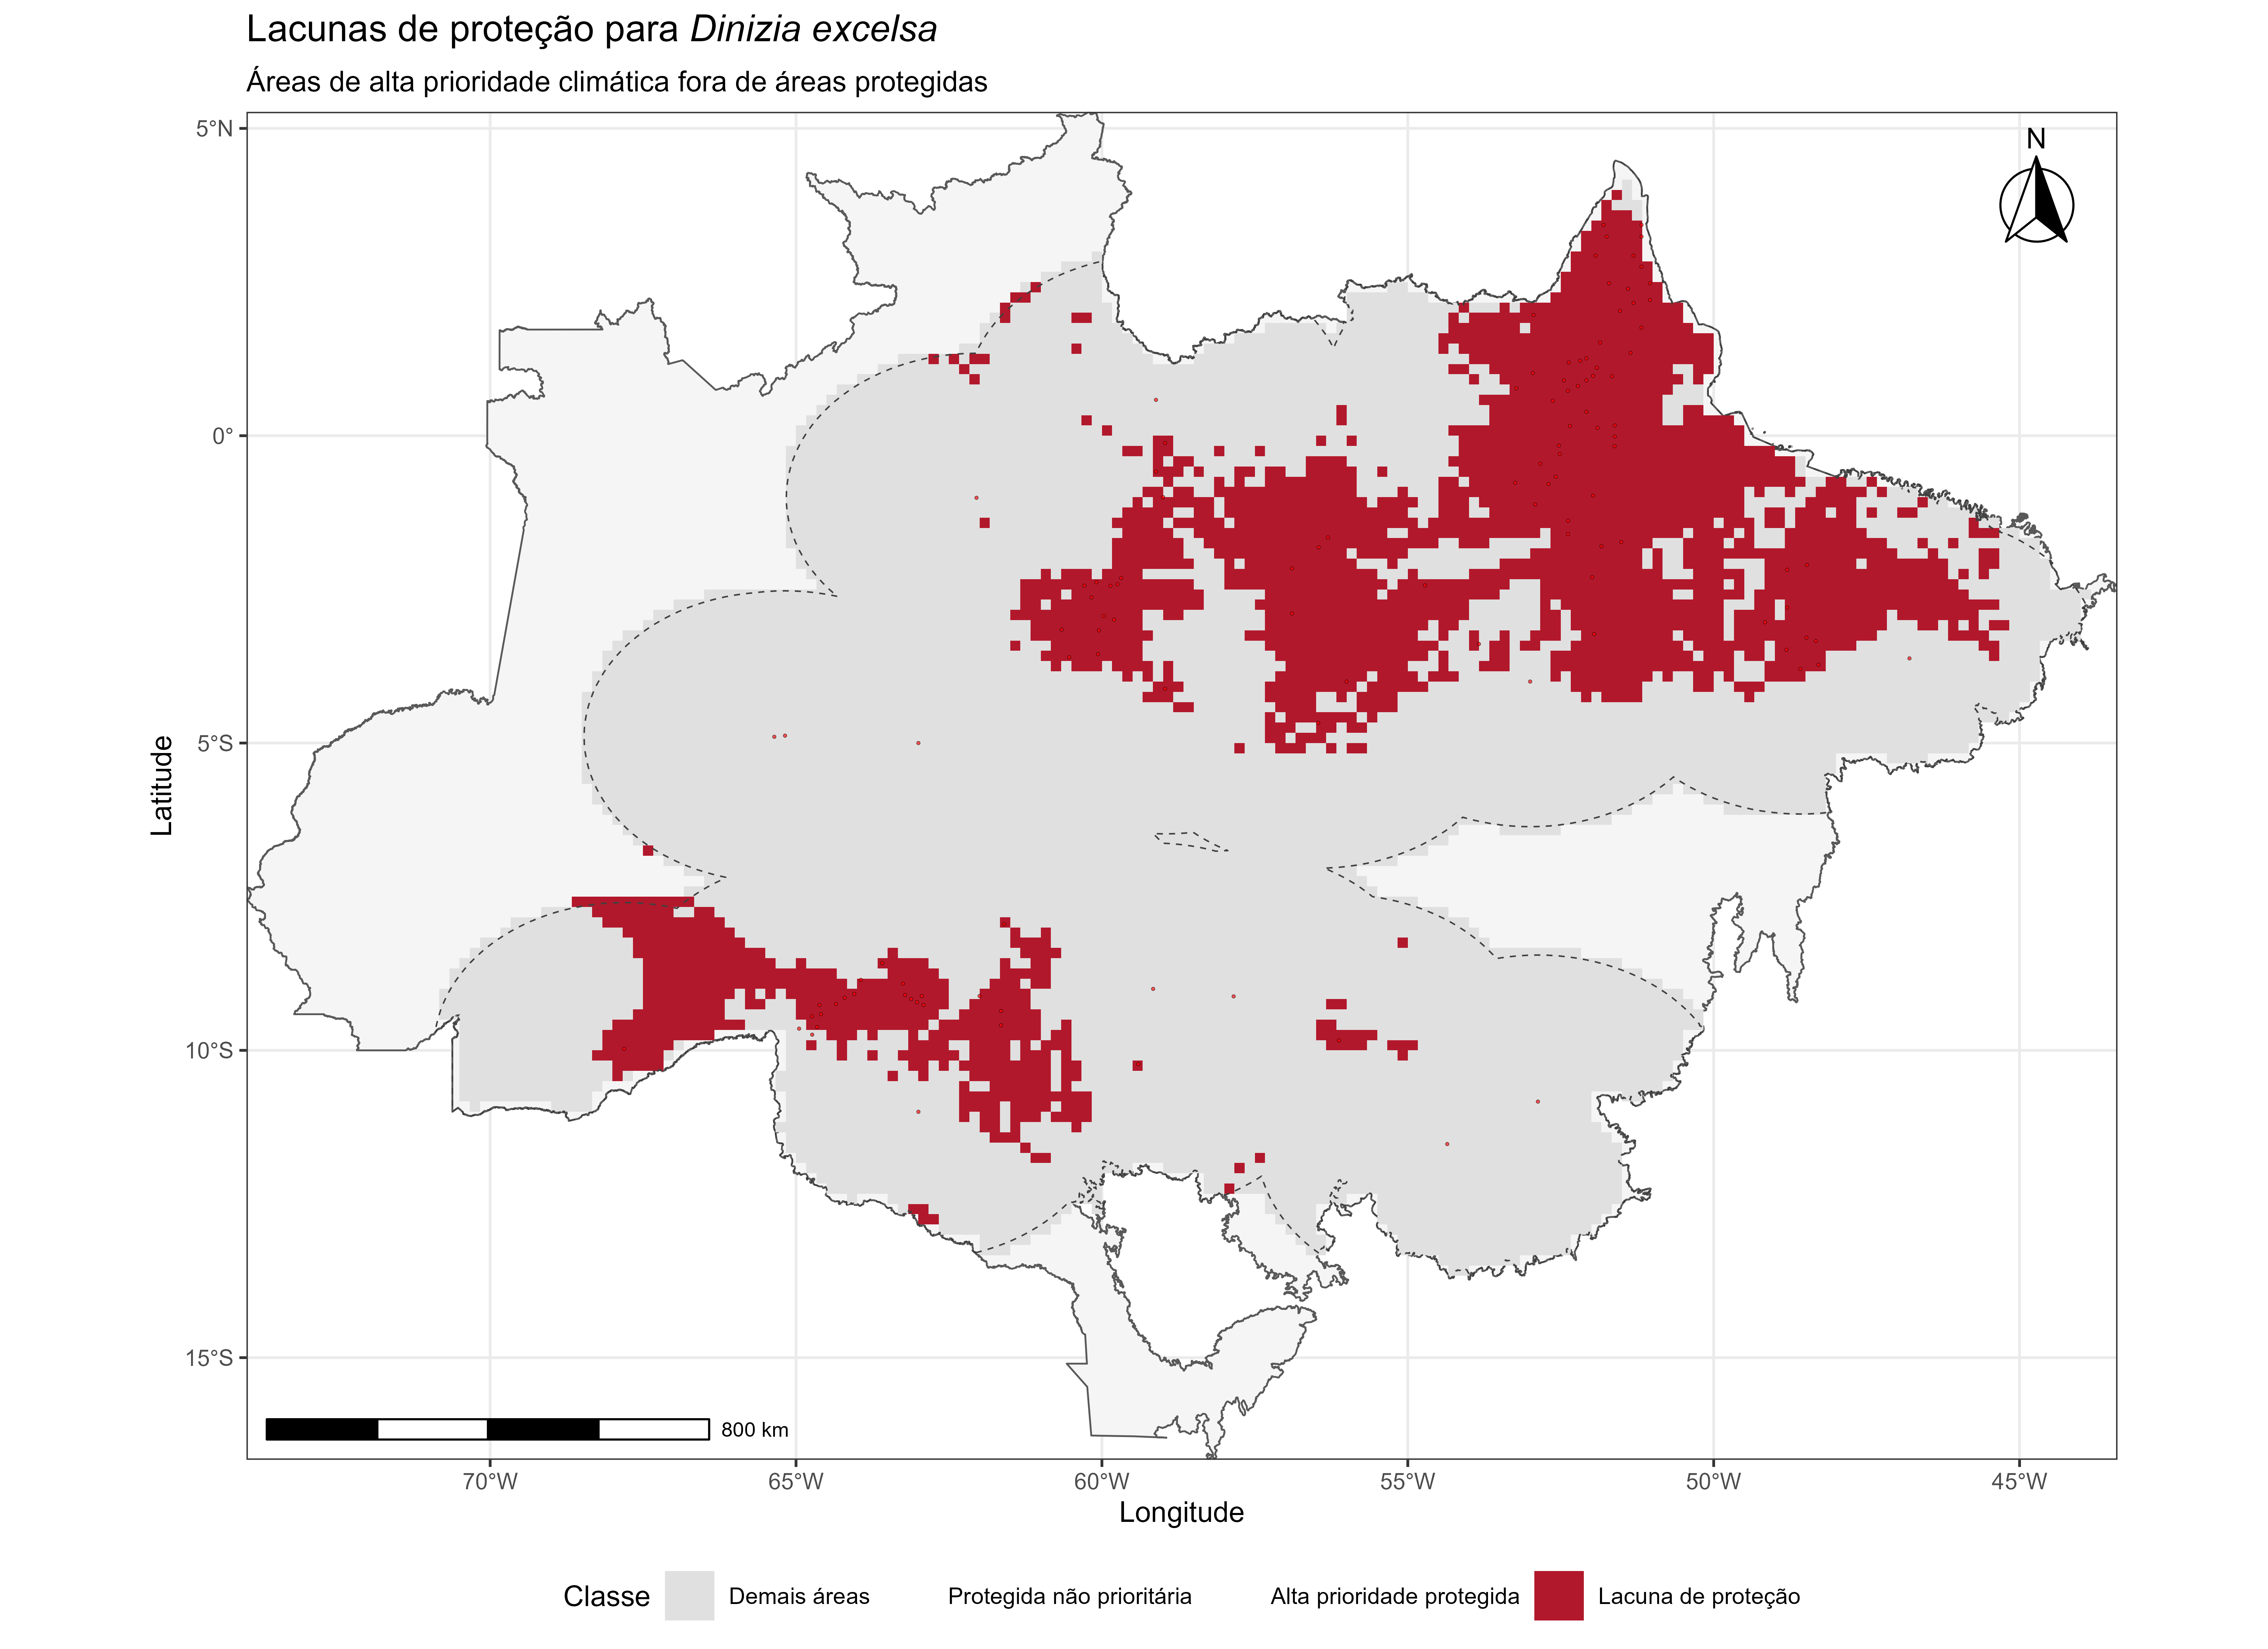
\includegraphics[width=0.90\textwidth]{figuras/unidade17/unidade17_lacunas_protecao.png}
	\caption{Lacunas potenciais de proteção para \textit{Dinizia excelsa}. Áreas prioritárias fora de unidades de conservação indicam possíveis regiões estratégicas para conservação.}
	\label{fig:unidade17_lacunas}
\end{figure}

\section{Mapa integrado de prioridade}

\rscriptfile{scripts/unidade17/07_prioridade_integrada_conservacao.R}

\begin{figure}[H]
	\centering
	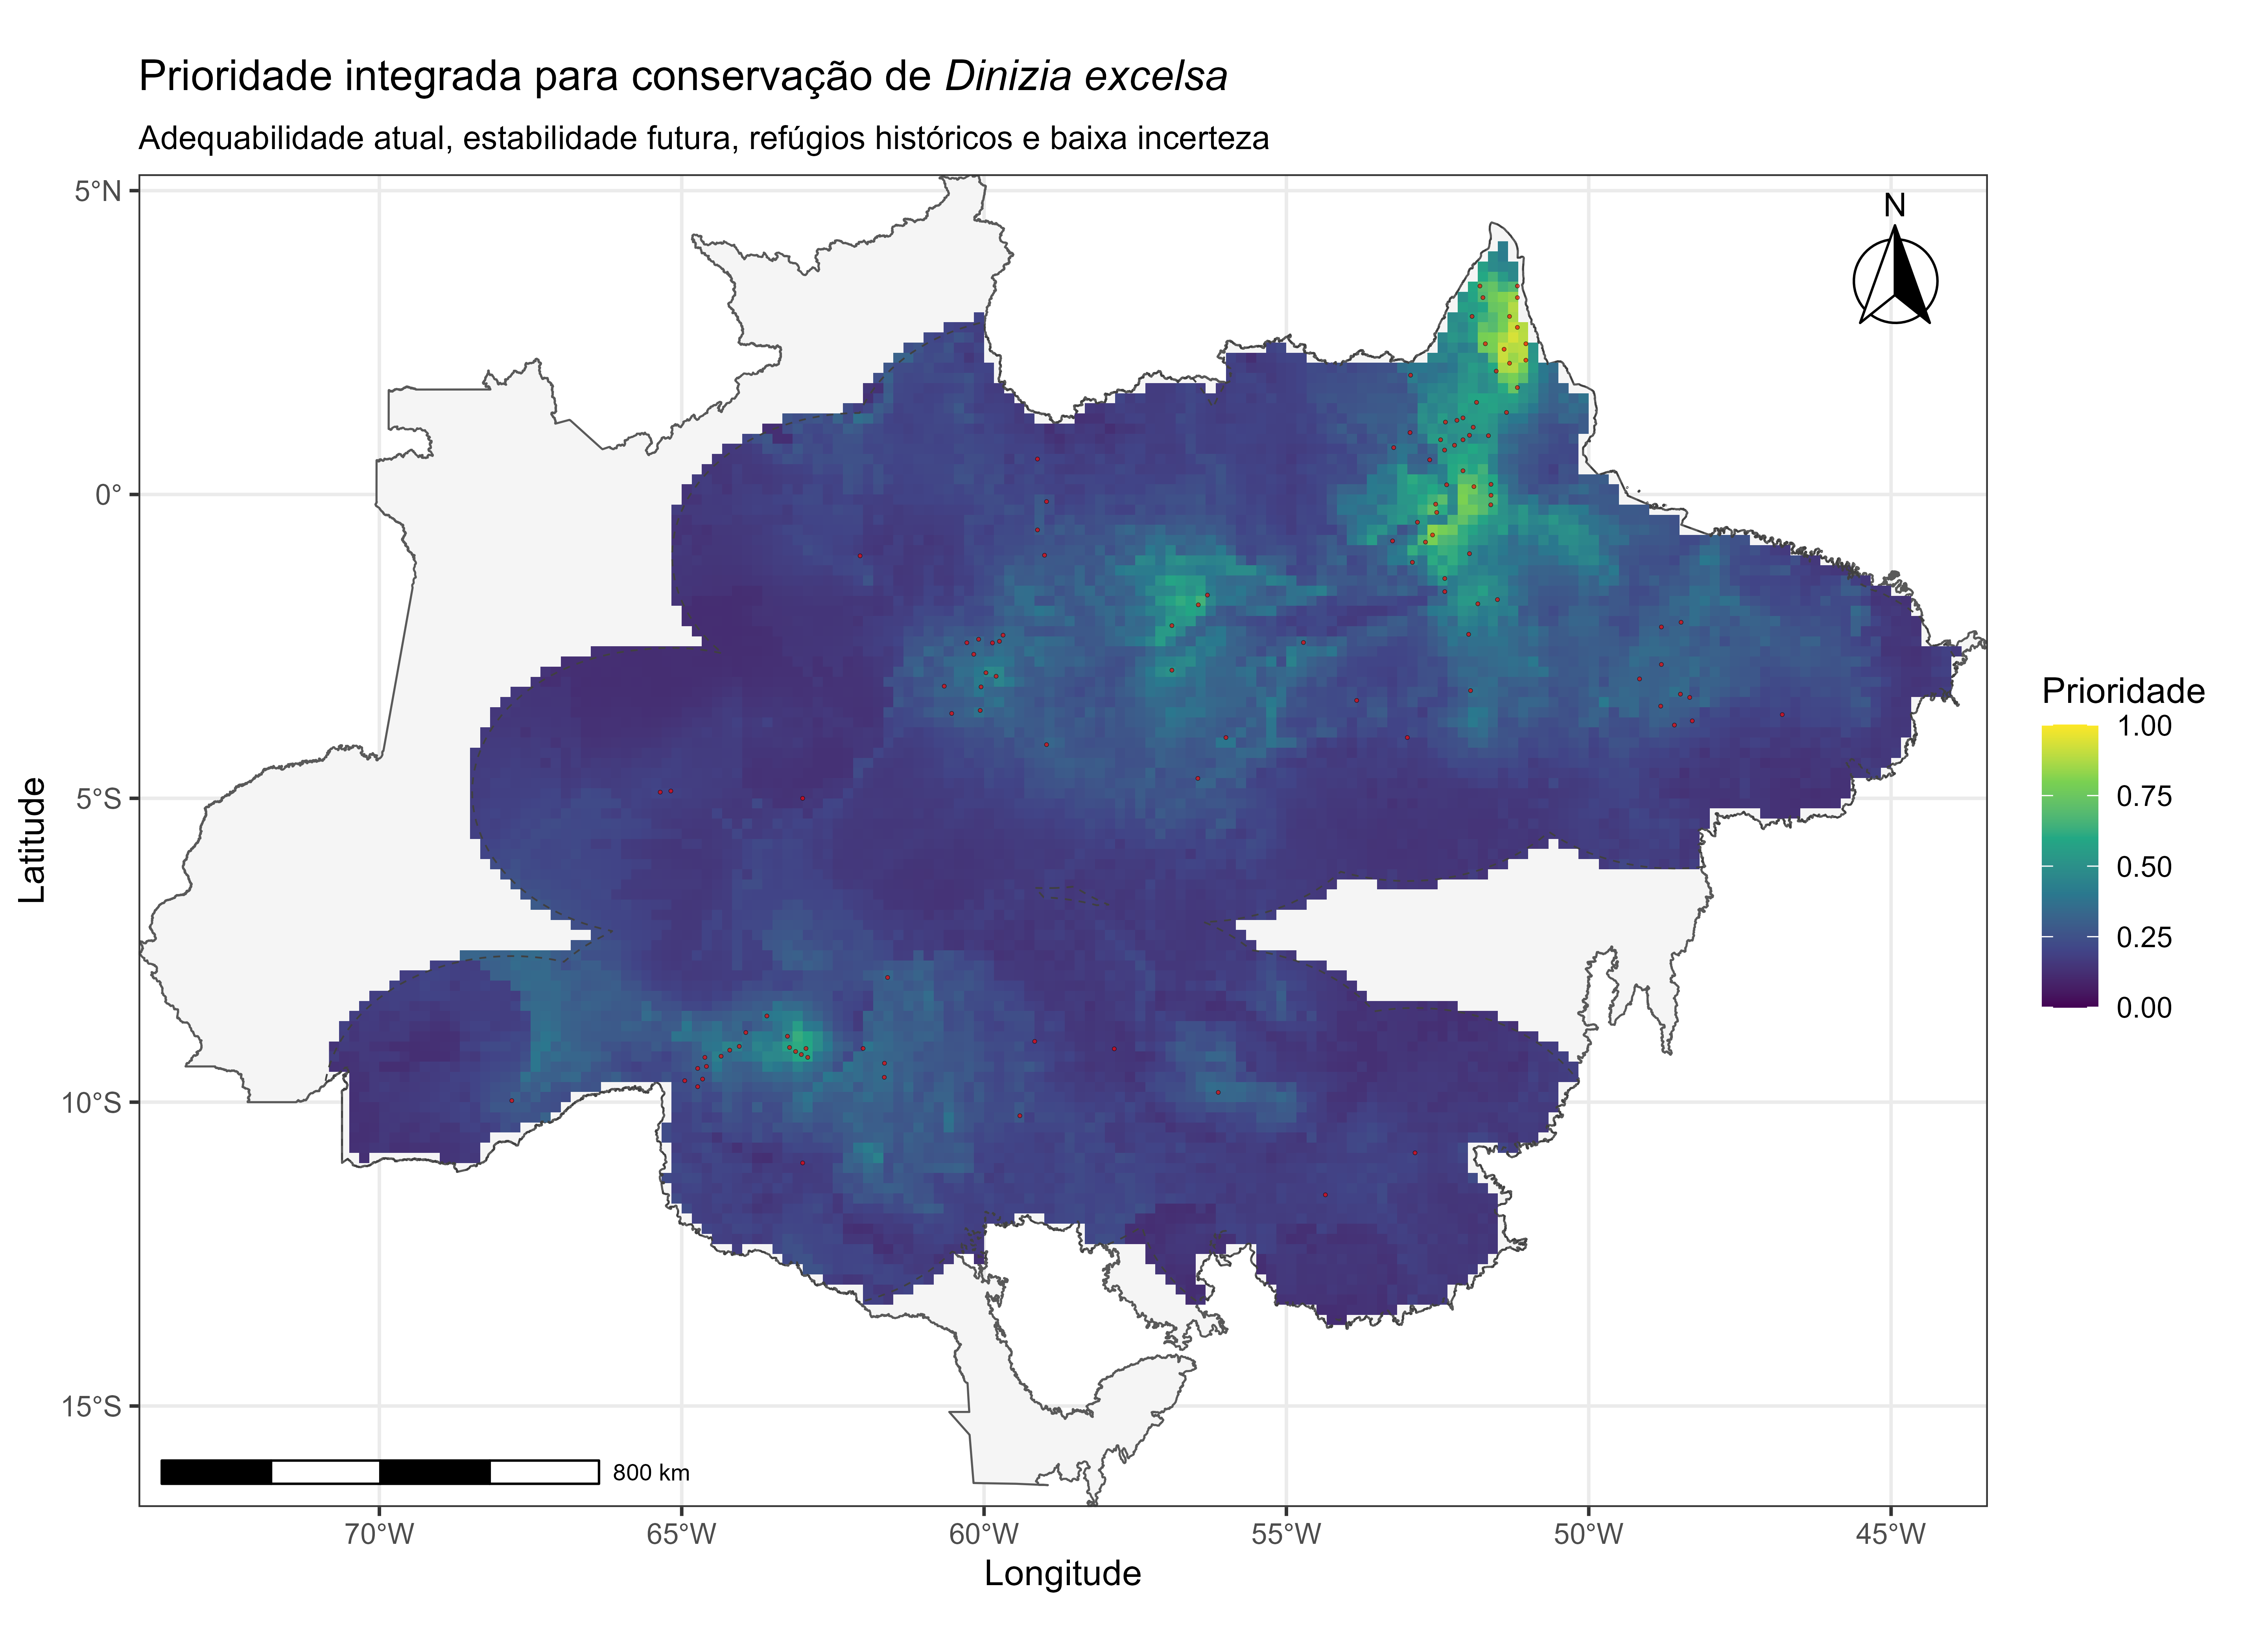
\includegraphics[width=0.90\textwidth]{figuras/unidade17/unidade17_prioridade_integrada.png}
	\caption{Mapa integrado de prioridade para conservação de \textit{Dinizia excelsa}.}
	\label{fig:unidade17_prioridade_integrada}
\end{figure}

\section{Síntese quantitativa}

\rscriptfile{scripts/unidade17/08_sintese_conservacao.R}

\begin{figure}[H]
	\centering
	\includegraphics[width=0.90\textwidth]{figuras/unidade17/unidade17_sintese_conservacao.png}
	\caption{Síntese quantitativa das classes de prioridade para conservação de \textit{Dinizia excelsa}.}
	\label{fig:unidade17_sintese}
\end{figure}

\section{Pipeline completo}

\rscriptfile{scripts/unidade17/09_pipeline_conservacao.R}

\section{Síntese da unidade}

A aplicação de SDM à conservação exige integração entre modelagem ecológica, mudanças climáticas, incerteza, estabilidade histórica e instrumentos territoriais de proteção. Para \textit{Dinizia excelsa}, a combinação desses elementos permite identificar áreas com maior potencial para conservação, monitoramento, restauração e planejamento estratégico.

\begin{conceito}[title={\faBook\quad Mensagem central}]
	A melhor aplicação conservacionista de SDM não é simplesmente mapear áreas adequadas, mas identificar áreas adequadas, estáveis, pouco incertas e estrategicamente relevantes para proteção da biodiversidade.
\end{conceito}

\section{Exercícios de fixação}

\begin{enumerate}
	\item Explique como SDM pode apoiar conservação de espécies arbóreas amazônicas.
	\item Por que áreas de alta adequabilidade e baixa incerteza são importantes?
	\item O que são lacunas de proteção?
	\item Como projeções futuras podem alterar prioridades de conservação?
	\item Por que estabilidade paleoclimática pode indicar possíveis refúgios?
	\item Como integrar SDM com áreas protegidas?
	\item Quais cuidados devem ser tomados antes de usar SDM em decisões públicas?
\end{enumerate}

\section{Síntese final da apostila}

Esta apostila encerra com uma mensagem central: Modelagem de Distribuição de Espécies não é apenas ajustar algoritmos. É um processo científico completo que conecta teoria ecológica, qualidade dos dados, hipóteses biogeográficas, variáveis ambientais, avaliação estatística, interpretação espacial, incerteza e conservação.

\begin{conceito}[title={\faBook\quad Mensagem final}]
	Um bom SDM não é aquele que apenas produz alto AUC. É aquele que possui dados confiáveis, hipóteses explícitas, área de calibração justificada, variáveis ecologicamente coerentes, modelos avaliados, incerteza comunicada e interpretação útil para ciência e conservação.
\end{conceito}

\section{Exercícios finais}

\begin{enumerate}
	\item Explique o fluxo completo de um projeto de SDM desde ocorrências até conservação.
	\item Por que a área acessível \(M\) influencia todo o pipeline?
	\item Compare os papéis de GLM, GAM, Random Forest e BRT no ensemble.
	\item Explique por que mapas de incerteza devem acompanhar mapas finais.
	\item Como projeções futuras podem apoiar decisões de conservação?
	\item Quais produtos finais devem ser entregues em um projeto reprodutível de SDM?
	\item Elabore um projeto de SDM para uma espécie amazônica de interesse ecológico ou conservacionista.
\end{enumerate}

% ============================================================
% UNIDADE 18
% ============================================================

%================================================
